\begin{flushleft}
	\section{\textcolor{cyan}{Conception et Réalisation du maison intelligente :}}
	\subsection{\textcolor{green}{Première solution utilisant le Bluetooth}}
	\subsubsection{\textcolor{blue}{Circuits électriques : Schéma, câblage et branchement}}
		\begin{figure}[h]
			\centering
			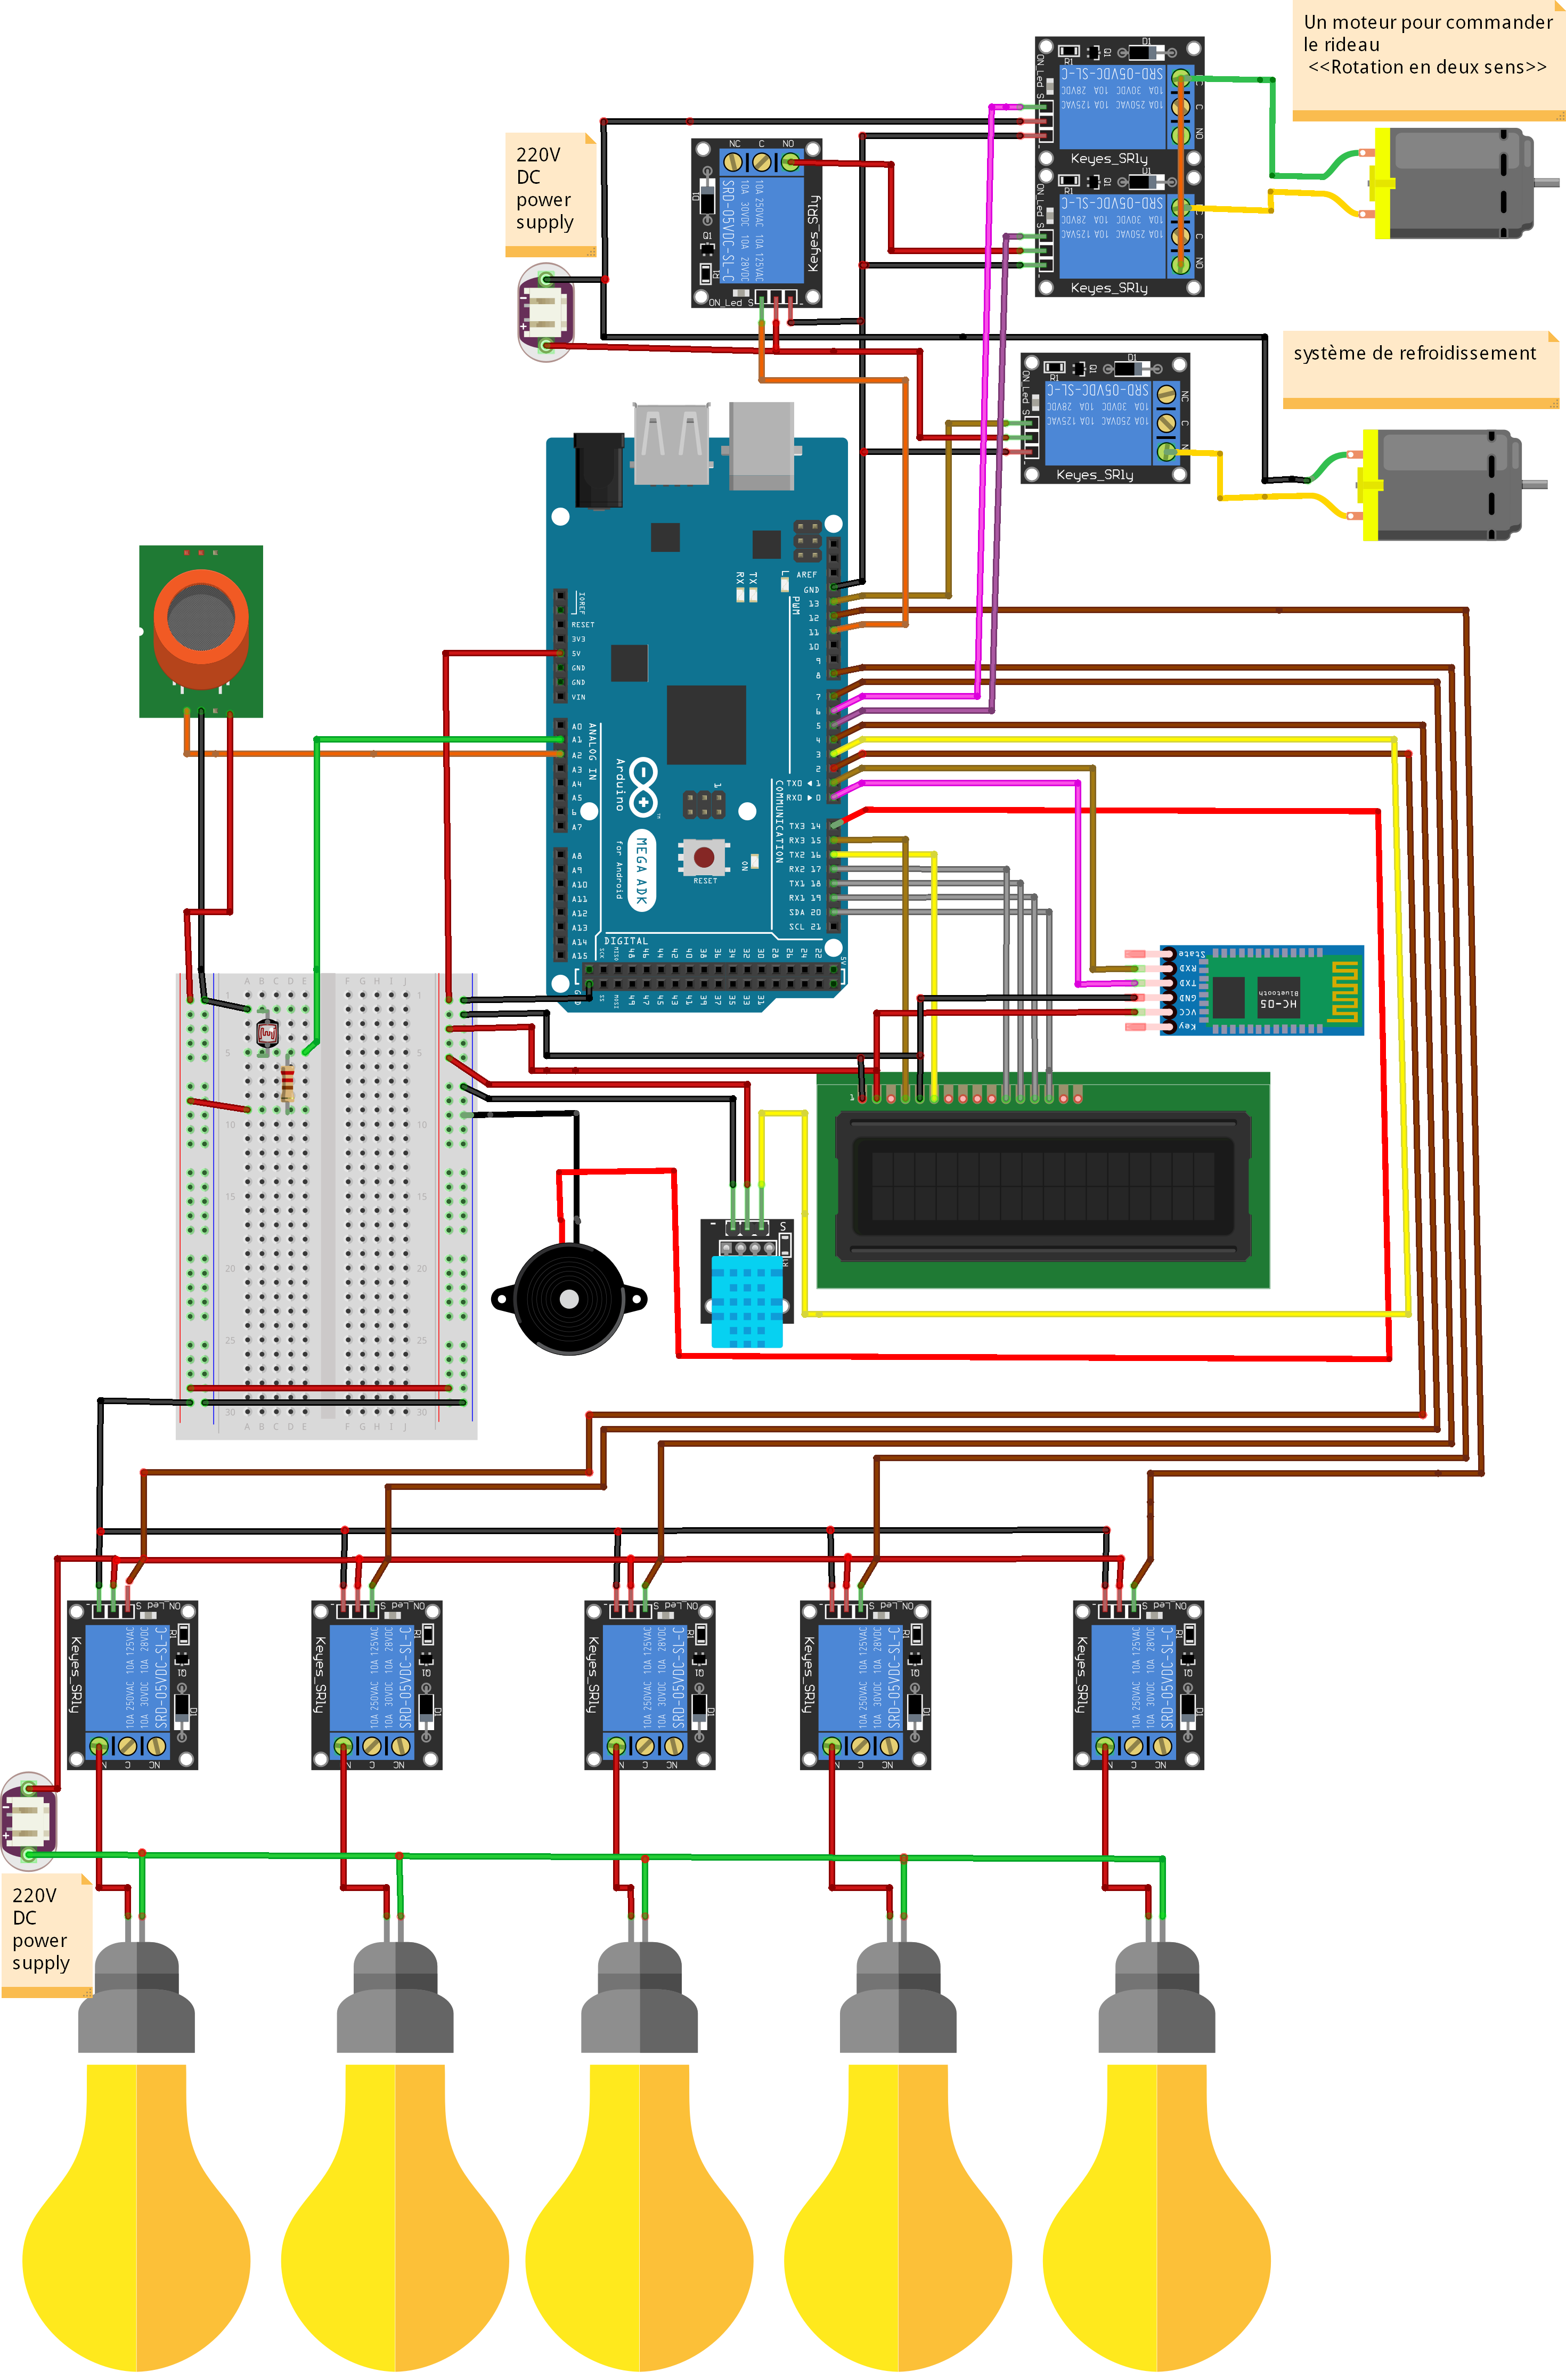
\includegraphics[width=0.7\textwidth]{chapitres/images/Simulation-Format-Fritzing_bb_bluetooth.png}
			\caption{Circuits électriques }
			\label{fig:labelname}
		\end{figure}
	\newpage
	\subsubsection{\textcolor{blue}{Conception de l'interface utilisateur avec Mit App Inventor :} }
					
					\begin{figure}[h]
						\centering
						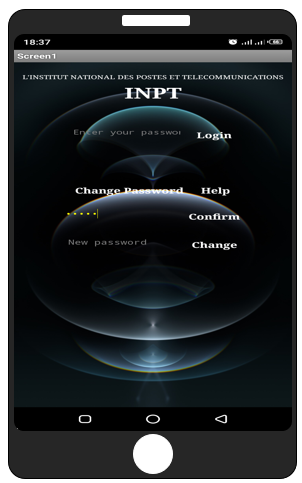
\includegraphics{chapitres/images/Fenetre1.PNG}
						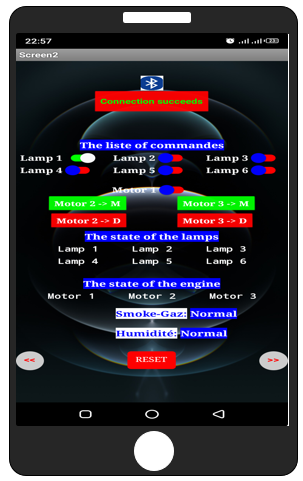
\includegraphics{chapitres/images/Fenetre2.PNG}
						\caption{l'interface utilisateur avec Mit App Inventor}
						\label{fig:labelname}
					\end{figure}
	\subsubsection{\textcolor{blue}{Réalisation finale du prototype :} }
	Notre prototype de maison connectée avec la technologie Bluetooth se compose d'une variété d'éléments soigneusement intégrés pour créer un système complet et fonctionnel. Nous avons utilisé une carte Arduino Mega comme base, et avons ajouté des fonctionnalités telles que des LED pour simuler le comportement des lampes, des moteurs pour simuler le système de refroidissement et le contrôle du rideau de la fenêtre, ainsi que des capteurs de température, d'humidité et de gaz pour surveiller l'environnement. Nous avons également inclus un afficheur LCD et une LDR pour réguler l'éclairage en fonction de la lumière ambiante (jour/nuit), ainsi qu'une application Android créée avec l'outil MIT App Inventor pour permettre un contrôle à distance facile et pratique du système.
					\begin{figure}[h]
						\centering
						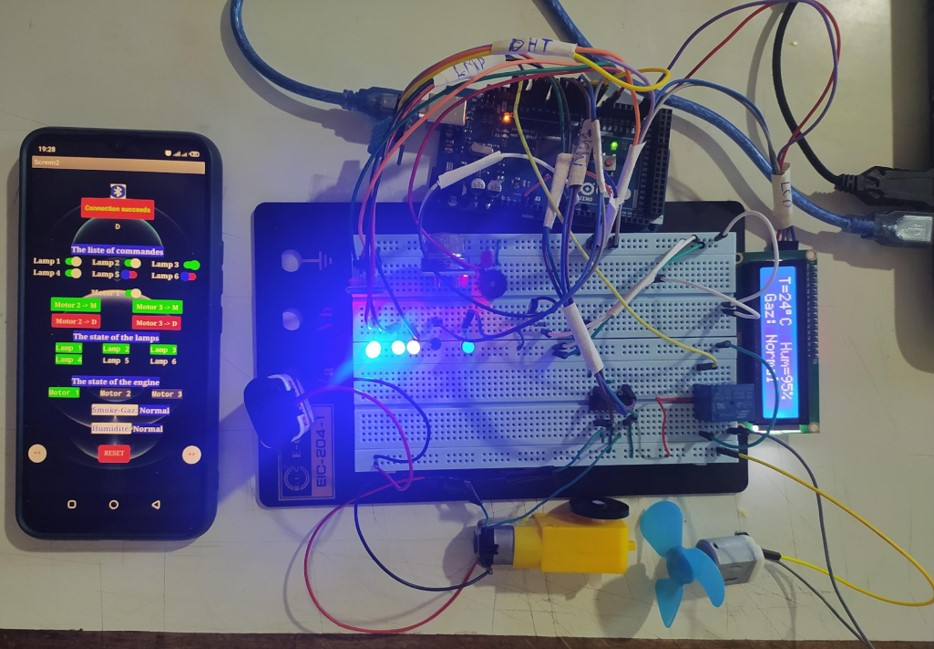
\includegraphics[width=0.9\textwidth]{chapitres/images/Picture1.jpg}
						\caption{Réalisation finale du prototype}
						\label{fig:labelname}
					\end{figure}
	
	
	\newpage
	\subsection{\textcolor{green}{Deuxième solution utilisant le WiFi}}
	\subsubsection{\textcolor{blue}{Circuits électriques : Schéma, câblage et branchement} }
		Notre prototype de maison connectée, équipé de la technologie WiFi, est composé d'une carte Arduino Mega et d'une carte ESP8266 pour le système. L'interface utilisateur est réalisée grâce à Node-RED, qui est relié à un broker Mosquitto installé sur un Raspberry Pi 4. Le prototype comprend également des LED pour simuler le comportement des lampes, un moteur pour simuler le système de refroidissement, un autre moteur pour simuler le contrôle du rideau de la fenêtre, ainsi que des capteurs de température, d'humidité et de détection de gaz. Nous avons également inclus un afficheur LCD et une LDR pour commander une lampe en fonction de la présence de lumière (jour/nuit).
			\begin{figure}[h]
				\centering
				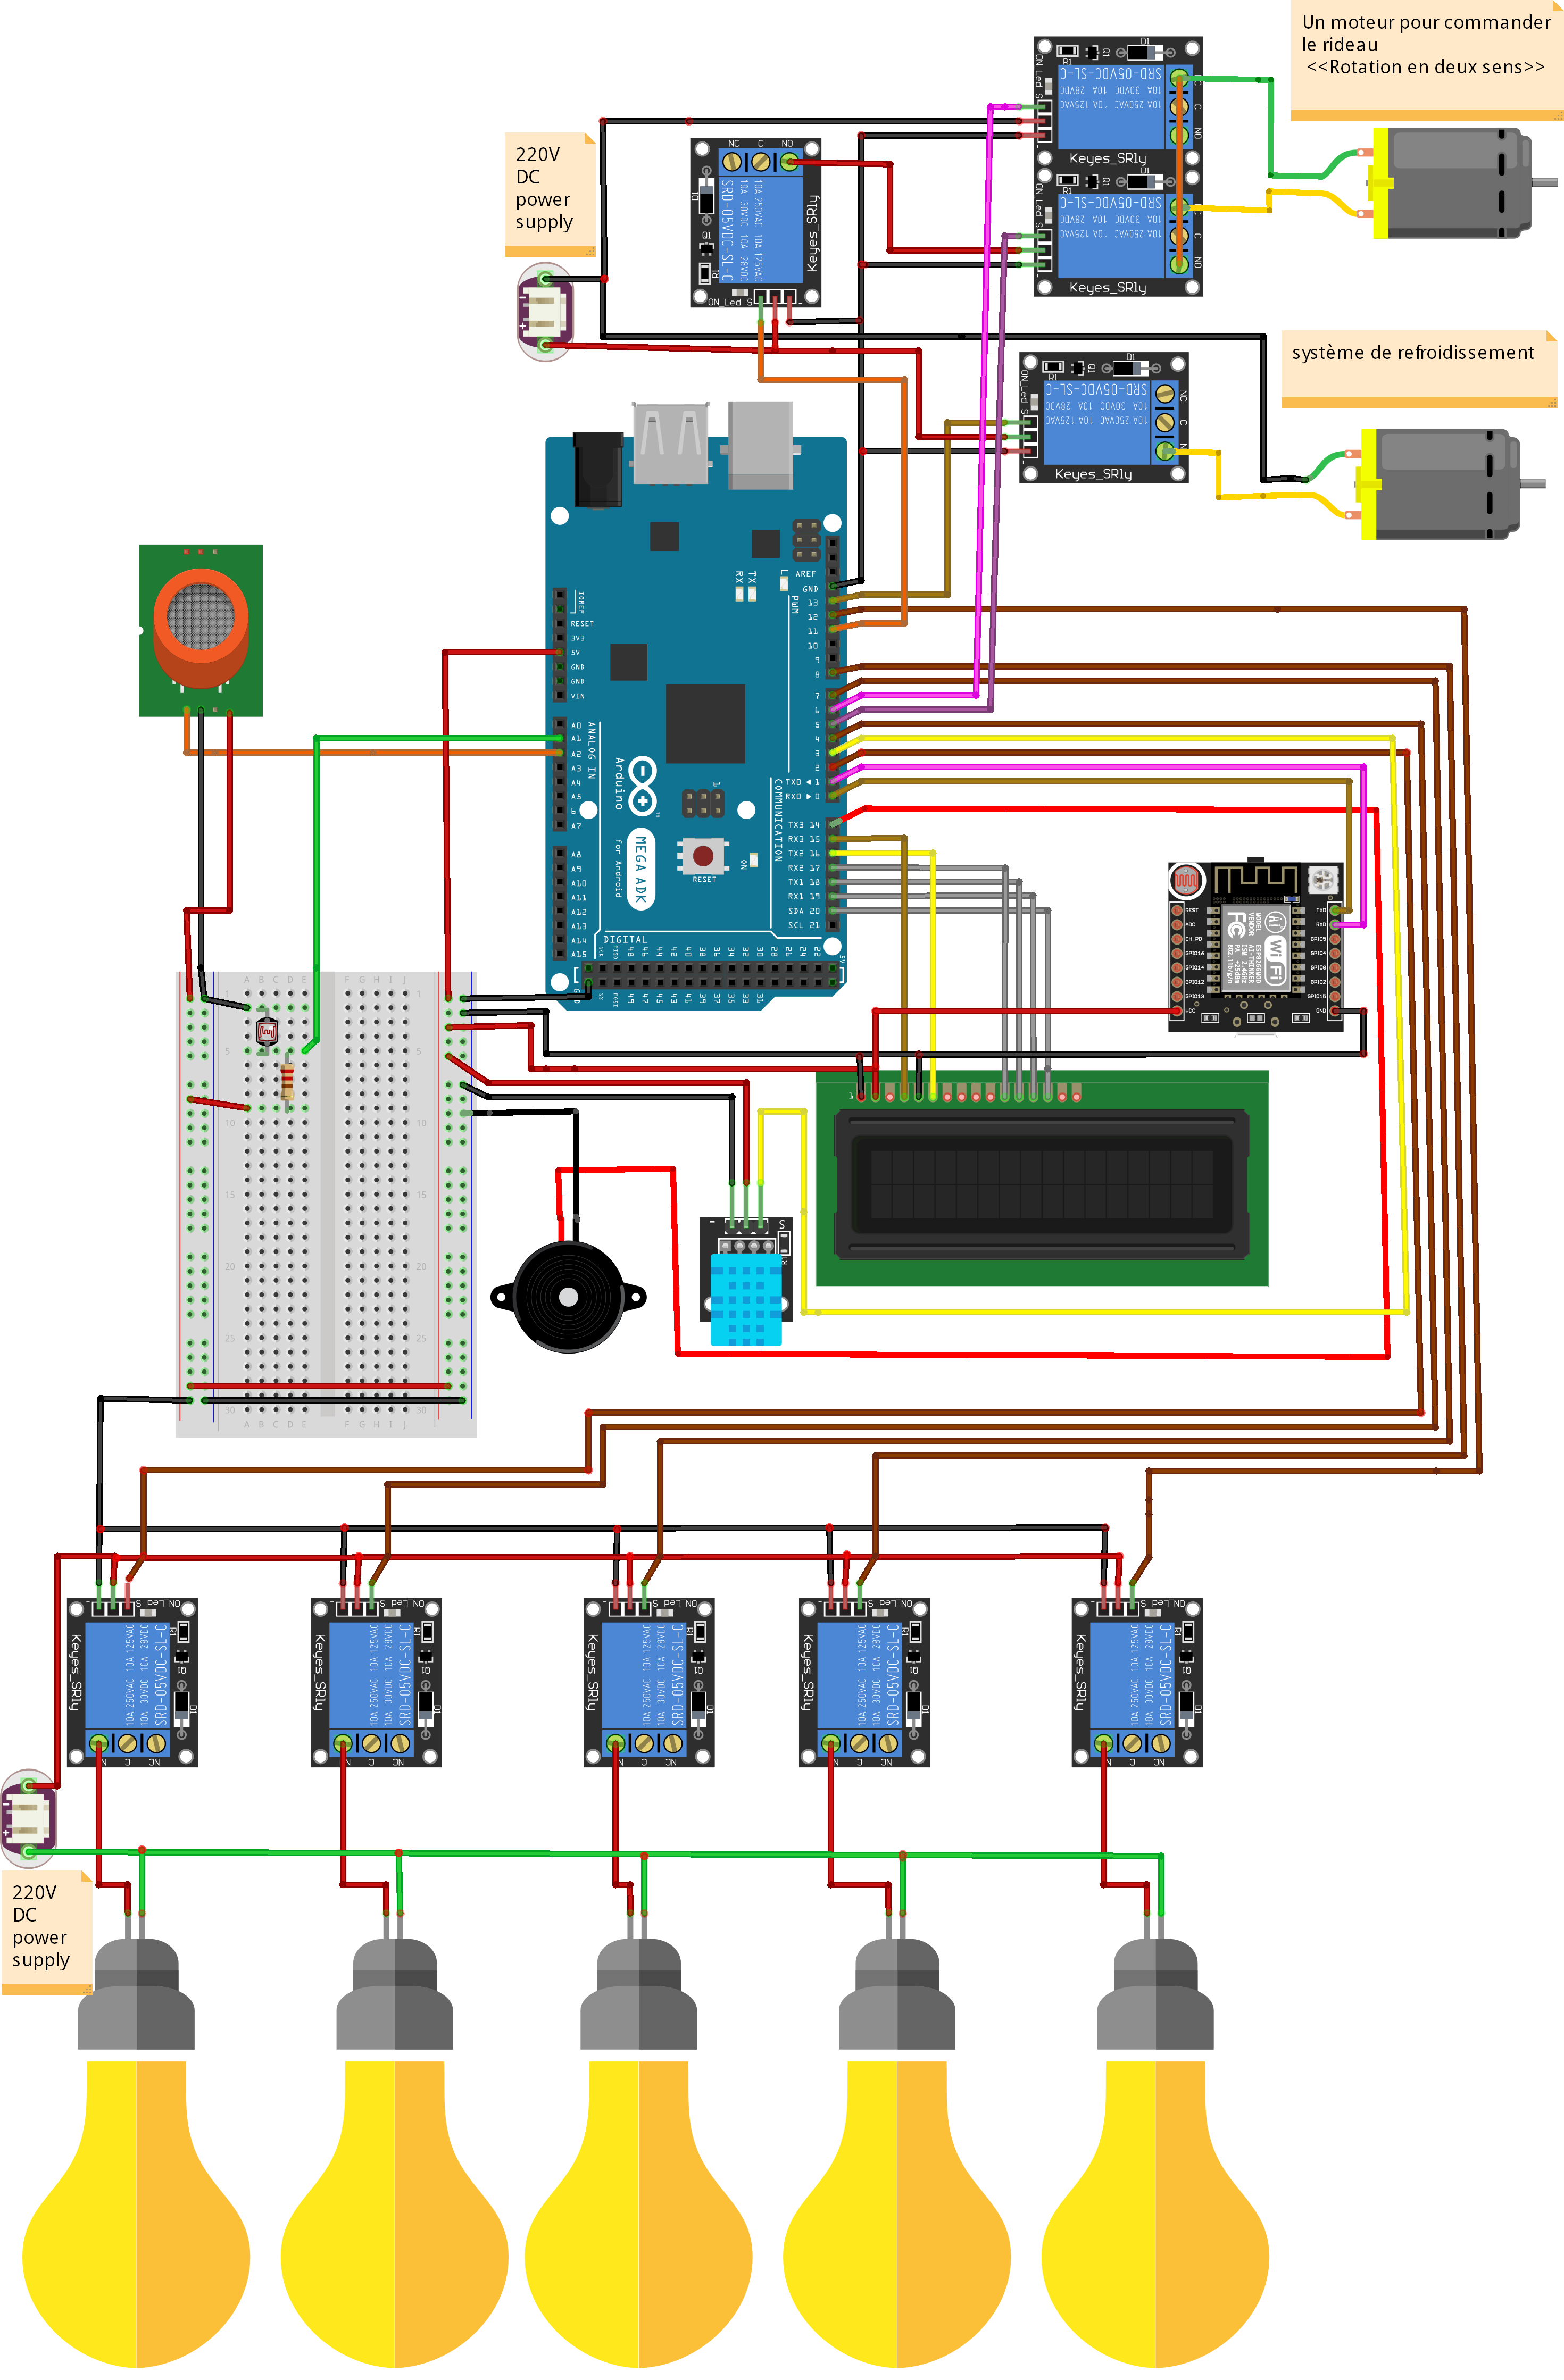
\includegraphics[width=0.6\textwidth]{chapitres/images/Simulation-Format-Fritzing_WiFi_bb.png}
				\caption{Circuits électriques}
				\label{fig:labelname}
			\end{figure}
		\newpage
	\subsubsection{\textcolor{blue}{Installation et démarrage du broker Mosquitto sur Raspberry Pi 4 :} }
				
				  \underline{sudo apt-get install -y mosquitto} : installera le broker Mosquitto sur votre Raspberry Pi. Cette commande installera également toutes les dépendances nécessaires.
				  
				  \underline{systemctl status mosquitto} : vérifiera le statut du service Mosquitto sur votre Raspberry Pi. Cette commande vous montrera si le service Mosquitto est en cours d'exécution ou non, et s'il y a des erreurs à corriger.
			\begin{figure}[h]
				\centering
				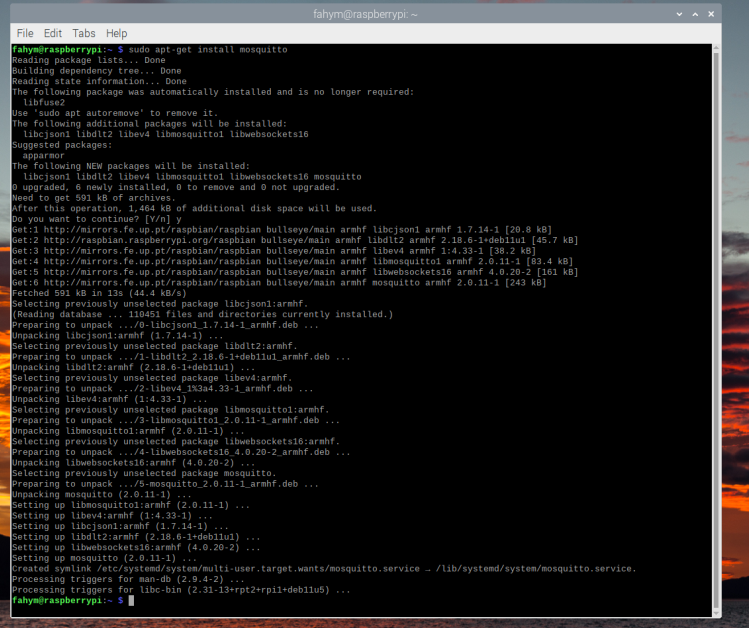
\includegraphics[width=0.7\textwidth]{chapitres/images/mosquitto1.PNG}
			\end{figure}
	 		\begin{figure}[h]
	 		\centering
	 		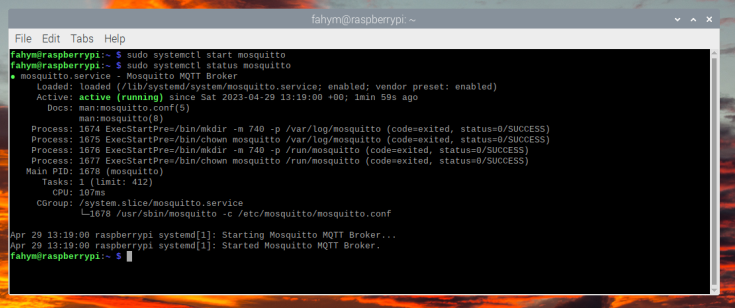
\includegraphics[width=0.7\textwidth]{chapitres/images/mosquitto2.PNG}
	 		\caption{Installation et démarrage du broker Mosquitto sur Raspberry Pi 4}
	 		\label{fig:labelname}
	 		\end{figure}
 		\newpage
	\subsubsection{\textcolor{blue}{Conception de l'interface utilisateur avec Node-RED :} }
		
		\begin{figure}[h]
			\centering
			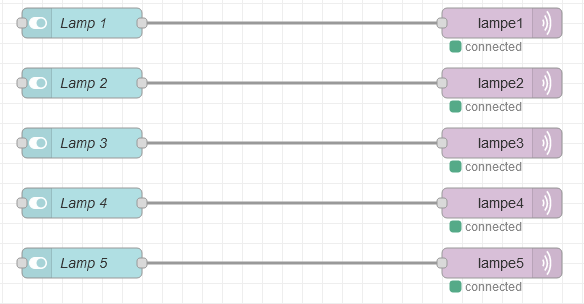
\includegraphics[width=0.7\textwidth]{chapitres/images/nodeRed2.png}
			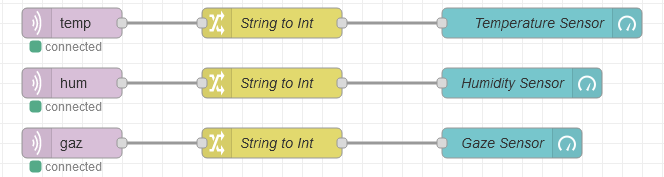
\includegraphics[width=0.7\textwidth]{chapitres/images/nodeRed1.png}
			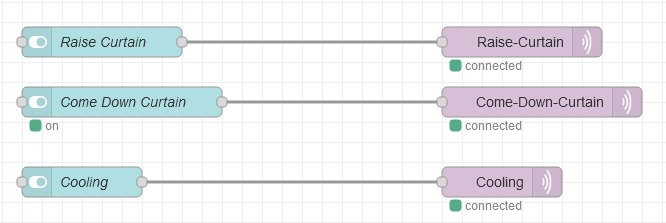
\includegraphics[width=0.7\textwidth]{chapitres/images/nodeRed3.png}
			\caption{L'interface utilisateur "Back end"}
			\label{fig:labelname}
		\end{figure}
		\begin{figure}[h]
			\centering
			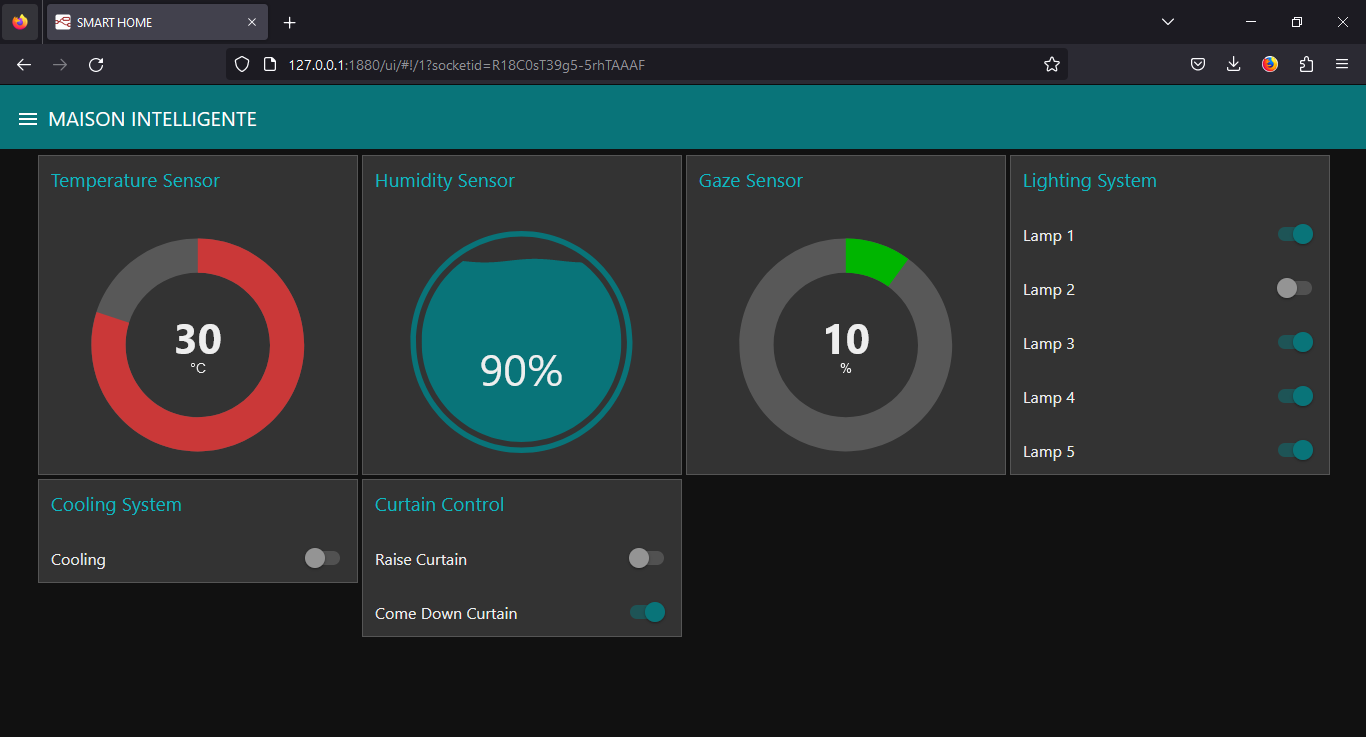
\includegraphics[width=0.7\textwidth]{chapitres/images/nodeRed4.png}
			\caption{L'interface utilisateur "Front end"}
			\label{fig:labelname}
		\end{figure}
	 \newpage
	\subsubsection{\textcolor{blue}{Réalisation finale du prototype :} }
		
				\begin{figure}[h]
					\centering
					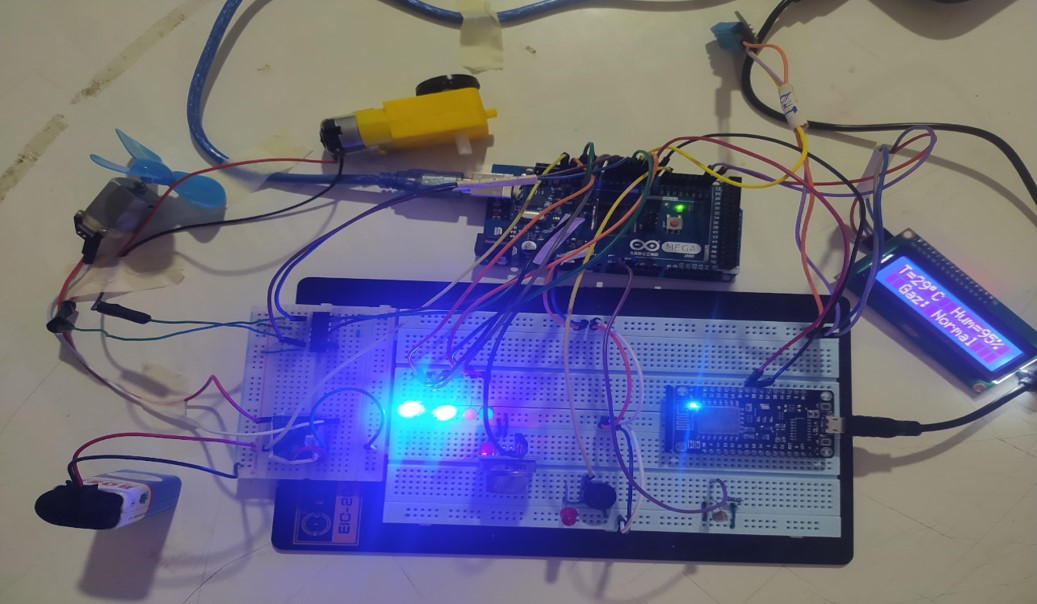
\includegraphics[width=0.7\textwidth]{chapitres/images/Picture2.jpg}
					\caption{Réalisation finale du prototype}
					\label{fig:labelname}
				\end{figure}
	\newpage
\end{flushleft}